\documentclass[11pt,a4paper]{article}
\usepackage{graphicx}
\usepackage[parfill]{parskip}
\usepackage[table]{xcolor}
\usepackage{fullpage}
\usepackage{array}
\newcolumntype{L}{>{\centering\arraybackslash}m{0.14\textwidth}}
\newcommand{\highPrio}{\cellcolor{green}High}
\newcommand{\medPrio}{\cellcolor{orange}Medium}
\newcommand{\lowPrio}{\cellcolor{yellow}Low}
\newcommand{\vLowPrio}{\cellcolor{yellow!50}Very Low}
\title{CodeBuzz}
\author{Team Gocky \\
    Craig McLaughlin, 1002524M \\
    Gordon Reid, 1002536R}
\begin{document}

\maketitle

\newpage

\section*{Abstract}

This report documents the specification and design of CodeBuzz,
a web-application for posting code snippets. The aim of the application is
to facilitate programming language learning by exposing beginners to
example programs written by industry experts and academics, and to
aid reuse by providing a store of solutions to commonly recurring
problems in software engineering. 
\newpage

\tableofcontents
\newpage

\section{Introduction}

CodeBuzz is a code snippet oriented application that allows users to submit code
in a variety of programming languages. This code is categorised based on the
code's language, and function (e.g. sorting algorithm). This categorisation
will allow other users to search for code snippets (e.g. Python Bubble Sort)
and have returned to them a list of matching snippets. These can be ordered
by popularity or user rating.

When a user views a code snippet they have the option to copy the snippet into
their clipboard or comment and rate the snippet.

The application can be used by novice coders looking for examples of common
language functions and can be used by intermediate/expert programmers to supply
their own examples, and rate others. Academics may also find this of use as
it can provide a convenient source of example code (which may or may not be
good code, both useful in this context).

\section{Functionality}

The site will operate similar to any collaborative web-based application
where users of the site need not be registered in order to contribute
to the site content.
The funcationality is detailed in the lists below. Next to each feature
is a parenthesised list of the user personas that are interested in
performing the task(s) afforded by the feature.
The following functionality is available to both registered and
non-registered users:

\begin{itemize}
\item Code snippets have their syntax highlighted.
\item Snippet hit rate/popularity.
\item Categorised code snippets by language and function.
\item Ability to search for code snippets based on language and
function.
\item Textual copy-to-clipboard.
\item Downloadable source code.
\item Links to other code snippets.
\end{itemize}

The following functionality is avaliable to only registered users:

\begin{itemize}
\item User can comment on the code snippets, e.g. reviewing the
correctness/usefulness of the code snippet.
\item User can rate a code snippet on a five star scale.
\item User profile which stores bookmarked snippets.
\item Social network integration.
\end{itemize}

\newpage

\section{Application Design Ideas}

\subsection{Wireframes}

Figure \ref{fig:anonsnippet} shows an anonymous snippet being posted by a
visitor to the website who has chosen not to log in. An example of the basic
layout and the syntax highlighting capabilities are shown in the figure.

Figure \ref{fig:joe} shows a logged in user posting a snippet. The user's
name is shown and there are also links to his profile, bookmarks, and other
user-specific data.

\begin{figure}
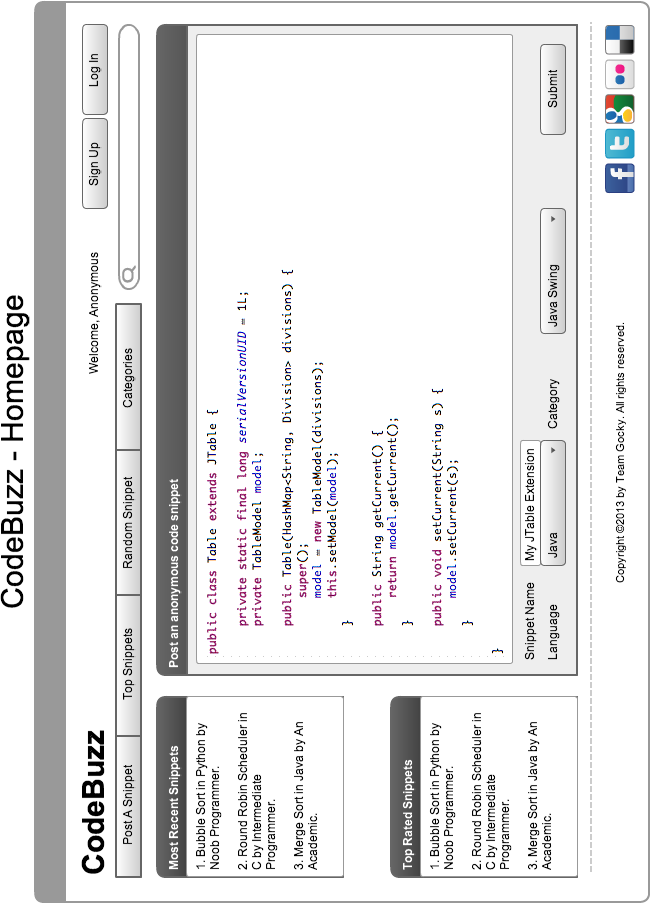
\includegraphics[width=\textwidth]{../imgs/homepageWireFrameGRHorz.png}
\caption{Anonymous snippet being posted.}
\label{fig:anonsnippet}
\end{figure}

\begin{figure}
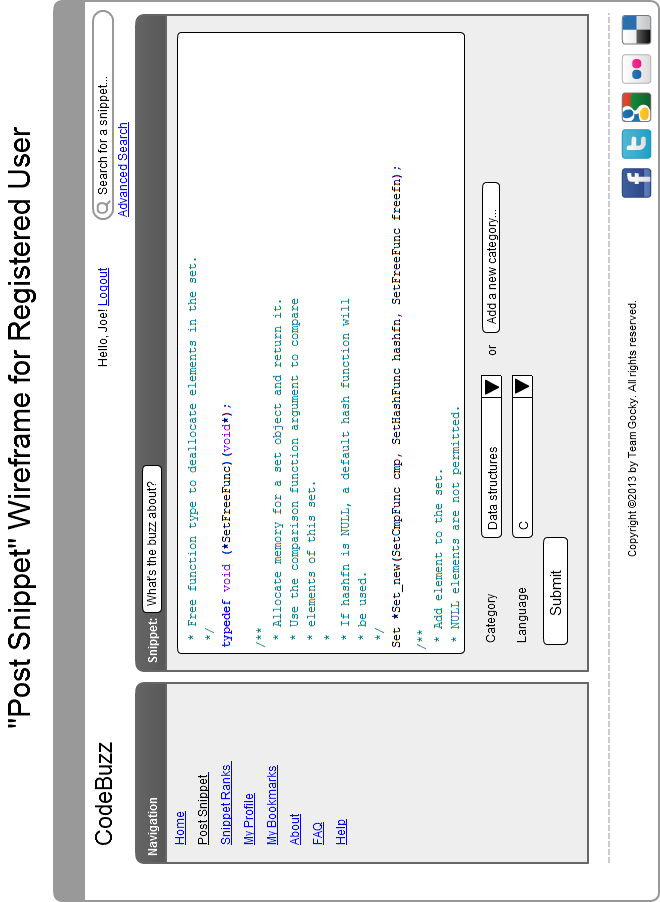
\includegraphics[width=\textwidth]{../imgs/CCodeSnippetHorz.png}
\caption{Joe's home screen with his code snippet}
\label{fig:joe}
\end{figure}

%subsection{Describe the user interface}
% Perhaps we need more wireframes!

\subsection{Design Goals}

The number one design goal is to make the user interface minimalist
such that the user is not overwhelmed by the application. As can be
seen in the two wire frames above, the application will have a simple
home screen both for registered and non-registered users. A finalised
version of the home screen is shown below (Need to talk about this).

\subsection{A Walk through: Submit a code snippet in C}

A simple walk through for the user Joe entering his C code snippet as
shown in Figure~\ref{fig:joe} is given below:

\begin{enumerate}
\item Joe logs in using his user details.
\item Joe is present with the home screen.
\item Joe selects the C programming language from the language drop-down
menu.
\item Joe proceeds to write his C code into the main window.
\item Joe selects the `Data Structures' category from the category
drop-down menu.
\item Joe is finished creating his code snippet and clicks the `Submit'
button.
\item Joe logs out.
\end{enumerate}

Note that the walk through above is applicable to a non-registered user
as well. For restrictions on non-registered users see
Section~\ref{sec:restrict}.

This walk through has highlighted a number of interactions between the
user and the application. It is important to note the order in which
the steps are carried out, particularly the selection of the
programming language and the entering of the code. The order is
important because the selection will dynamically set the syntax
highlighting mode in the application to the language specified.
The text that the user then enters is highlighted according to the
language selected. This highlighting is performed on-demand. % (!)
However, the application will not enforce this ordering on the user.

\newpage

\section{Personas}

\subsection{Barry: The Noob Programmer}
% CMCL went with some suggestions from
% http://www.steptwo.com.au/papers/kmc_personas/index.html
% eliminating the personal details and just detailing the following:
% user’s goals, behaviours, likes and dislikes. 

Barry is sixteen, studying a computing based course and is looking to
learn a particular language. Barry's programming ability is, at best,
amateur. He relys heavily on introductory texts and Internet forums
since his school does not provide learning materials for the language
of interest.

\subsubsection{Goals}

\begin{itemize}
\item Finding code snippets to perform a specific programming task,
e.g. reading from a file.
\item Looking for code on a particular language.
\item To download/copy the code snippet for integration into their
program.
\item Comment on a snippet to ask questions if understanding is low.
\end{itemize}

\subsubsection{Behaviours}

\begin{itemize}
\item Curiosity towards others code for inspiration for their own code
development. Looking for ideas on, `How it's done', etcetera.
\item Impatient regarding the `slowness' of their learning, wanting to
get their application up and running as soon as possible. Quick and
dirty.
\end{itemize}

\subsubsection{Likes}

\begin{itemize}
\item Syntax-highlighted environments that help his noobish brain
comphrehend what is going on.
% We should just insult our personas continuously:
%\item Dubious scripts that he downloads and runs immediately in the
%hope that it will work without even scanning it for viruses because he
%is a noob.
\item When code works out of the box.
\item Easy-to-read code, using simple constructs and ideas so that it
is simple to digest.
\end{itemize}

\subsubsection{Dislikes}

\begin{itemize}
\item Being unable to find the desired code snippet, or one which is
too complex/advanced for their current abilities.
\item Being overwhelmed by large number of advanced search capabilities.
\end{itemize}

\newpage

\subsection{Intermediate Programmer}

This person has recently completed a course which heavily involved programming.
They have some working knowledge in a few languages and are eager to pick up
more and expand their knowledge of their current languages. They are able to
pick up new languages easier because they understand the underlying, basic
principles of programming.

\subsubsection{Goals}

\begin{itemize}
\item Find code snippets to perform a programming task they are unfamiliar
with in a language that they are familiar with.
\item Find code snippet in a language they are not familiar with.
\item Post snippets to have them rated by individuals with more experience than
themselves.
\end{itemize}

\subsubsection{Behaviours}

\begin{itemize}
\item Curiosity towards others code for inspiration for their own code
development. Looking for ideas on `How it's done', etcetera.
\item Interested in how well their own code compares to expert programmers
code.
\end{itemize}

\subsubsection{Likes}

\begin{itemize}
\item Picking up new programming concepts.
\item Picking up new programming languages.
\item Helping others with less experience, they still remember when they were
in that position.
\end{itemize}

\subsubsection{Dislikes}

\begin{itemize}
\item Being unhelpfully shot down for minor coding errors or inefficiencies.
\item Being unable to seek help from experts.
\end{itemize}

\newpage

\subsection{The Academic}

This person is a University Professor, College Professor, or possibly high
school teacher teaching a computing-based course. They contribute code for
their research area, courses they teach, and own personal interest. They are
also interested in the code their students produce to check on individuals
progress and to monitor lab attendance and participation.

\subsubsection{Goals}

\begin{itemize}
\item Looking for crowd-sourced examples of how, or how not to, code a certain
programming function for use in class.
\item Use as a platform for student-submitted code that can be peer-reviewed.
\item Comment/rate student-submitted code as part of the learning process.
\item Upload examples of standard/optimised solutions to coding problems.
\end{itemize}

\subsubsection{Behaviours}

\begin{itemize}
\item Looking to aid the learning of students and others in their programming.
\item Interested in submitting high quality code for re-use and to contribute
to the Open Source community.
\end{itemize}

\subsubsection{Likes}

\begin{itemize}
\item The ability to review code snippets.
\item Being able to provide sample high-quality, working solutions.
\end{itemize}

\subsubsection{Dislikes}

\begin{itemize}
\item Poor quality code being passed off as working.
\item Students not keeping up with work given.
\end{itemize}

\newpage

\subsection{Experienced Programmer}

This person works, or used to work, in industry on medium-large commercial
software projects. They have working knowledge of multiple programming
languages and are well versed in different paradigms and making use of good
software engineering concepts such as design patterns.

\subsubsection{Goals}

\begin{itemize}
\item Scout out potential future job candidates.
\item Suggest optimisations and changes to a user's submitted code.
\end{itemize}

\subsubsection{Behaviours}

\begin{itemize}
\item Becomes frustrated with other's mistakes however wishes to aid the
learning of individuals so they can become more proficient in programming.
\end{itemize}

\subsubsection{Likes}

\begin{itemize}
\item Seeing potential in other people for future job roles.
\end{itemize}

\subsubsection{Dislikes}

\begin{itemize}
\item Poor quality code being passed off as working.
\item Repeatedly being asked simple questions or seeing the same fundamental
errors.
\item Beginners that do not RTFM.
\end{itemize}

\newpage

\section{User Needs Matrix}

\begin{table}[h]
\begin{tabular}{*{6}{|L}|}
\hline
I want to... & Overall Priority & Noob Programmer & Intermediate Programmer
& The Academic & Experienced Programmer\\
\hline
Search solution code & \highPrio & \highPrio & \highPrio & \medPrio 
& \lowPrio \\
\hline
Contribute quality code & \highPrio & \lowPrio & \medPrio & \highPrio & 
\highPrio \\
\hline
Rate a code snippet & \highPrio & \lowPrio & \medPrio & \highPrio & \medPrio \\
\hline
Comment on a snippet & \highPrio & \medPrio & \medPrio & \highPrio & 
\lowPrio \\
\hline
Bookmark a snippet & \medPrio & \medPrio & \medPrio & \highPrio & \medPrio \\
\hline
Submit code for review & \medPrio & \highPrio & \medPrio & \vLowPrio &
\vLowPrio \\
\hline
Share code externally & \lowPrio & \medPrio & \medPrio & \vLowPrio &
\vLowPrio \\
\hline
View highly rated code & \medPrio & \highPrio & \highPrio & \medPrio &
\lowPrio \\
\hline
View code hit count & \lowPrio & \lowPrio & \lowPrio & \vLowPrio & \vLowPrio \\
\hline
\end{tabular}
\end{table}

\end{document}  
